\documentclass[12pt, a4paper]{article}
\usepackage[utf8]{inputenc}
\usepackage[T1]{fontenc}
\usepackage[brazil]{babel}
\usepackage{amsmath, amsfonts, amssymb}
\usepackage{graphicx}
\usepackage{geometry}
\usepackage{setspace}
\usepackage{indentfirst}
\usepackage{caption}
\usepackage{subcaption}
\usepackage{cite}
\usepackage{listings}
\usepackage{xcolor}
\usepackage{booktabs}
\usepackage{array}
\usepackage{multirow}
\usepackage{fancyhdr}
\usepackage{hyperref}
\usepackage{float}
\usepackage{enumitem}
\usepackage{tcolorbox}
\tcbuselibrary{skins,breakable}
\usepackage{tikz}
\usetikzlibrary{shapes.geometric,arrows.meta,positioning,fit,backgrounds,calc}

\geometry{left=3cm, top=3cm, right=2cm, bottom=2cm}
\onehalfspacing

% ─── Cores ────────────────────────────────────────────────────────────────────
\definecolor{codegray}{rgb}{0.96,0.96,0.96}
\definecolor{codeblue}{rgb}{0.0,0.0,0.6}
\definecolor{codegreen}{rgb}{0.0,0.45,0.0}
\definecolor{codepurple}{rgb}{0.5,0.0,0.6}
\definecolor{aquacolor}{rgb}{0.0,0.50,0.55}
\definecolor{boxblue}{rgb}{0.88,0.93,0.98}
\definecolor{boxgreen}{rgb}{0.88,0.97,0.88}
\definecolor{boxyellow}{rgb}{1.0,0.98,0.88}

% ─── Listagens ────────────────────────────────────────────────────────────────
\lstset{
  basicstyle=\ttfamily\footnotesize,
  backgroundcolor=\color{codegray},
  frame=single, rulecolor=\color{gray!50},
  breaklines=true,
  keywordstyle=\color{codeblue}\bfseries,
  commentstyle=\color{codegreen}\itshape,
  stringstyle=\color{codepurple},
  numbers=left, numberstyle=\tiny\color{gray}, numbersep=6pt,
  tabsize=2, showspaces=false, showstringspaces=false,
  captionpos=b,
}
\lstdefinelanguage{SystemVerilog}[]{Verilog}{
  morekeywords={logic,typedef,enum,unique,unique0,priority,always_comb,always_ff,
                always_latch,interface,modport,clocking,program,package,import,
                bit,byte,shortint,int,longint,real,string,void,automatic,
                assert,assume,cover,property,sequence,endproperty,endsequence,
                task,endtask,function,endfunction,module,endmodule,
                parameter,localparam,input,output,inout,wire,reg,begin,end},
}

% ─── Caixas de destaque ───────────────────────────────────────────────────────
\newtcolorbox{conceitobox}[1][]{
  colback=boxblue, colframe=aquacolor!80!black,
  fonttitle=\bfseries, title=#1, breakable, before upper=\setlength{\parskip}{4pt}
}
\newtcolorbox{resultadobox}[1][]{
  colback=boxgreen, colframe=codegreen!70!black,
  fonttitle=\bfseries, title=#1, breakable
}
\newtcolorbox{unidadebox}[1][]{
  colback=boxyellow, colframe=orange!70!black,
  fonttitle=\bfseries\small, title=#1, breakable,
  before upper=\footnotesize
}

% ─── Cabecalho ────────────────────────────────────────────────────────────────
\pagestyle{fancy}\fancyhf{}
\rhead{\footnotesize Unidade 5 | Cap. 1 -- MUX 4:1 -- PADIS / Microeletronica 2026}
\lhead{\footnotesize Matheus Serrao Uchoa | Matricula: 22052633}
\rfoot{\thepage}

\hypersetup{colorlinks=true, linkcolor=aquacolor!80!black,
            citecolor=codeblue, urlcolor=codeblue}

\begin{document}

%% ─── CAPA ──────────────────────────────────────────────────────────────────
\begin{titlepage}
\begin{center}
  {\Large\bfseries Capacitacao Profissional em Microeletronica}\\[0.15cm]
  {\large\bfseries PADIS -- Programa de Apoio ao Desenvolvimento Tecnologico\\
   da Industria de Semicondutores}\\[1.6cm]

  {\large\bfseries Matheus Serrao Uchoa \quad Matricula: 22052633}\\[1.8cm]

  {\LARGE\bfseries RELATORIO TECNICO\\[0.3cm]
   Unidade 5 $|$ Capitulo 1 -- Multiplexador (MUX)\\
   de 4 Entradas em SystemVerilog}\\[1.0cm]

  {\Large\bfseries Projeto e Verificacao Funcional de um MUX 4-para-1\\
   Parametrico com Testbench Automatizado}\\[1.6cm]

  \vfill
  {\normalsize\textbf{Disciplina:} Design de Circuitos Integrados -- CI Amazonia / PADIS}\\[0.1cm]
  {\normalsize\textbf{Professor:} Alexandre Almeida}\\[0.3cm]
  {\normalsize Manaus -- AM \quad Maio de 2026}
\end{center}
\end{titlepage}

\setcounter{page}{1}
\tableofcontents
\newpage

%% ─── 1. INTRODUCAO ─────────────────────────────────────────────────────────
\section{Introducao}

A presente atividade consiste no projeto e na verificacao de um multiplexador 4-para-1
(MUX 4:1) utilizando a linguagem de descricao de hardware SystemVerilog (IEEE~1800-2012).
O escopo compreende a modelagem estrutural de um circuito combinacional parametrizado,
empregando blocos procedurais (\texttt{always\_comb}) e estruturas condicionais
(\texttt{unique case}) para o roteamento de dados. Adicionalmente, engloba o
desenvolvimento de um ambiente de simulacao (\textit{testbench}) executado localmente
com o simulador Icarus Verilog v12, para a injecao de estimulos logicos e a validacao
do \textit{design} por meio da geracao de logs de console e da analise grafica de
sinais (formas de onda em arquivo \texttt{.vcd}).

\begin{conceitobox}[O que e um Multiplexador?]
Um Multiplexador (\textbf{MUX}) e um circuito combinacional que atua como uma
``chave seletora'': dadas $N$ entradas de dados e $\log_2 N$ linhas de selecao,
ele direciona exatamente \textbf{uma} das entradas para a saida unica, com base
no valor binario das linhas de selecao. Para $N=4$, sao necessarios 2 bits de
selecao, cobrindo os estados $S \in \{00, 01, 10, 11\}$.

\medskip
Multiplexadores sao blocos fundamentais em sistemas digitais: sao usados em
barramentos de dados, arbitros de acesso, circuitos de roteamento em FPGAs
(\textit{Field-Programmable Gate Arrays}) e no interior de multiplexadores
maiores (cascateamento).
\end{conceitobox}

%% ─── 2. OBJETIVOS ──────────────────────────────────────────────────────────
\section{Objetivos}

O objetivo primario desta atividade consiste em projetar e verificar funcionalmente
um MUX de 4 entradas para 1 saida, empregando a linguagem SystemVerilog. A execucao
visa consolidar o entendimento tecnico sobre:

\begin{itemize}
  \item Arquitetura de modulos SystemVerilog, declaracao de portas e parametros
        (\texttt{\#(parameter int DATA\_WIDTH = 8)}).
  \item Manipulacao de tipos de dados vetorizados (\texttt{logic [DATA\_WIDTH-1:0]}).
  \item Aplicacao pratica do bloco procedimental \texttt{always\_comb} para modelagem
        de logica combinacional sem latch.
  \item Uso do construtor \texttt{unique case} para garantia de cobertura completa
        dos estados e verificacao pelo sintetizador.
  \item Desenvolvimento de um \textit{testbench} com verificacao automatica PASS/FAIL
        para validar exaustivamente todas as combinacoes de entrada e selecao.
  \item Geracao e interpretacao de formas de onda em formato VCD
        (\textit{Value Change Dump}).
\end{itemize}

\begin{unidadebox}[Conexao com o Curso -- Unidade 5 / Capitulo 1: MUX]
Este trabalho implementa diretamente o conteudo da Unidade~5, Capitulo~1, que
trata de circuitos combinacionais de roteamento. O MUX 4:1 e a base para blocos
mais complexos como decodificadores, demultiplexadores e unidades logicas e
aritmeticas (ULA). O parametro \texttt{DATA\_WIDTH} demonstra como o SystemVerilog
permite \textit{design} reutilizavel e escalavel, um requisito de nivel industrial.
\end{unidadebox}

%% ─── 3. MATERIAIS E EQUIPAMENTOS ───────────────────────────────────────────
\section{Materiais e Equipamentos Utilizados}

\begin{table}[H]
\centering
\small
\caption{Ferramentas e tecnologias utilizadas na atividade.}
\label{tab:ferramentas}
\begin{tabular}{p{3.5cm}p{3.0cm}p{6.5cm}}
\toprule
\textbf{Ferramenta} & \textbf{Versao} & \textbf{Funcao}\\
\midrule
SystemVerilog & IEEE 1800-2012 & Linguagem de descricao de hardware (HDL) \\
Icarus Verilog & v12.0 (iverilog) & Compilador e simulador RTL open-source \\
VVP Runtime & v12.0 & Motor de simulacao (executa o binario compilado) \\
GTKWave / EPWave & -- & Visualizador de formas de onda VCD \\
Python 3 + Matplotlib & 3.x & Geracao de graficos de formas de onda para o relatorio \\
\bottomrule
\end{tabular}
\end{table}

A modelagem do DUT (\textit{Design Under Test}) e do \textit{testbench} foram
codificados inteiramente em SystemVerilog IEEE~1800-2012. A compilacao e a
simulacao RTL (\textit{Register-Transfer Level}) foram executadas localmente
via \texttt{iverilog -g2012}. Para visualizacao das formas de onda, o arquivo
\texttt{dump.vcd} gerado pela simulacao foi analisado com o visualizador EPWave.

%% ─── 4. FUNDAMENTOS TEORICOS ───────────────────────────────────────────────
\section{Fundamentos Teoricos}

\subsection{Tabela-Verdade do MUX 4:1}

A Tabela~\ref{tab:verdade} apresenta a funcionalidade completa do multiplexador 4-para-1.
Com duas linhas de selecao ($S_1$, $S_0$), o circuito cobre $2^2 = 4$ combinacoes possiveis.

\begin{table}[H]
\centering
\caption{Tabela-verdade do MUX 4:1. $Y$ assume o valor da entrada selecionada.}
\label{tab:verdade}
\begin{tabular}{cccc}
\toprule
$S_1$ & $S_0$ & $S$ (decimal) & $Y$ (saida)\\
\midrule
0 & 0 & 0 & $D_0$ \\
0 & 1 & 1 & $D_1$ \\
1 & 0 & 2 & $D_2$ \\
1 & 1 & 3 & $D_3$ \\
\bottomrule
\end{tabular}
\end{table}

A expressao booleana equivalente para 1~bit de cada entrada e:
\begin{equation}
  Y = \overline{S_1}\,\overline{S_0}\,D_0
    + \overline{S_1}\,S_0\,D_1
    + S_1\,\overline{S_0}\,D_2
    + S_1\,S_0\,D_3
  \label{eq:mux_bool}
\end{equation}

\subsection{Diagrama de Blocos}

A Figura~\ref{fig:mux_block} apresenta o diagrama de blocos do MUX 4:1 parametrico
com \texttt{DATA\_WIDTH}~bits de largura de dados.

\begin{figure}[H]
\centering
\begin{tikzpicture}[
  port/.style={rectangle, draw=gray!60, fill=gray!8, rounded corners=2pt,
               text width=1.6cm, align=center, minimum height=0.6cm, font=\small},
  mux/.style={rectangle, draw=aquacolor!80!black, fill=aquacolor!10,
              rounded corners=4pt, text width=3.0cm, align=center,
              minimum height=4.8cm, font=\bfseries\small},
  arr/.style={-Stealth, thick, color=aquacolor!80!black},
  lbl/.style={font=\footnotesize}
]
% MUX body
\node[mux] (m) at (0,0) {MUX\\4:1\\[0.6cm]\footnotesize DATA\_WIDTH\\bits};

% Entradas D0..D3
\node[port, left=2.2cm of m, yshift= 1.8cm] (d0) {$D_0$};
\node[port, left=2.2cm of m, yshift= 0.6cm] (d1) {$D_1$};
\node[port, left=2.2cm of m, yshift=-0.6cm] (d2) {$D_2$};
\node[port, left=2.2cm of m, yshift=-1.8cm] (d3) {$D_3$};

% Saida Y
\node[port, right=2.2cm of m] (y) {$Y$};

% Selecao S
\node[port, below=1.6cm of m] (s) {$S[1:0]$};

% Arrows entradas
\draw[arr] (d0.east) -- node[above, lbl]{[DW-1:0]} ++(0.6,0) |- ([yshift= 1.8cm]m.west);
\draw[arr] (d1.east) -- ++(0.6,0) |- ([yshift= 0.6cm]m.west);
\draw[arr] (d2.east) -- ++(0.6,0) |- ([yshift=-0.6cm]m.west);
\draw[arr] (d3.east) -- node[below, lbl]{[DW-1:0]} ++(0.6,0) |- ([yshift=-1.8cm]m.west);

% Arrow saida
\draw[arr] (m.east) -- node[above, lbl]{[DW-1:0]} (y.west);

% Arrow selecao
\draw[arr] (s.north) -- node[right, lbl]{[1:0]} (m.south);
\end{tikzpicture}
\caption{Diagrama de blocos do MUX 4-para-1 parametrico. \texttt{DW} = \texttt{DATA\_WIDTH}.
As entradas $D_0$--$D_3$ e a saida $Y$ possuem largura configuravel. As linhas de
selecao $S[1:0]$ definem qual entrada e roteada para $Y$.}
\label{fig:mux_block}
\end{figure}

%% ─── 5. RESULTADOS EXPERIMENTAIS ───────────────────────────────────────────
\section{Resultados Experimentais}

\subsection{Codigo SystemVerilog -- Modulo \texttt{mux\_4\_to\_1}}

O modulo abaixo implementa o MUX 4:1 parametrico em SystemVerilog. O parametro
\texttt{DATA\_WIDTH} (padrao: 8~bits) permite reutilizar o mesmo modulo para
diferentes larguras de barramento (8, 16, 32 bits etc.) sem modificacao do codigo.

O bloco \texttt{always\_comb} garante que a logica e puramente combinacional:
qualquer variacao em \texttt{d0..d3} ou \texttt{s} propaga imediatamente para
\texttt{y}, sem dependencia de clock. O construtor \texttt{unique case} acrescenta
verificacao de cobertura completa dos estados pelo sintetizador -- qualquer
combinacao de \texttt{s} nao listada gera um aviso em tempo de sintese, evitando
latches ocultos.

\begin{lstlisting}[language=SystemVerilog,
  caption={Modulo \texttt{mux\_4\_to\_1.sv} -- MUX 4-para-1 parametrico em SystemVerilog.},
  label={lst:mux}]
module mux_4_to_1 #(
    parameter int DATA_WIDTH = 8      // largura dos dados (padrao: 8 bits)
)(
    input  logic [DATA_WIDTH-1:0] d0, // entrada 0: selecionada quando s = 2'b00
    input  logic [DATA_WIDTH-1:0] d1, // entrada 1: selecionada quando s = 2'b01
    input  logic [DATA_WIDTH-1:0] d2, // entrada 2: selecionada quando s = 2'b10
    input  logic [DATA_WIDTH-1:0] d3, // entrada 3: selecionada quando s = 2'b11
    input  logic [1:0]            s,  // linhas de selecao (2 bits)
    output logic [DATA_WIDTH-1:0] y   // saida unica
);

    // always_comb = logica combinacional pura (sem clock, sem latch)
    always_comb begin
        unique case (s)
            2'b00:   y = d0;
            2'b01:   y = d1;
            2'b10:   y = d2;
            2'b11:   y = d3;
            default: y = '0;  // estado seguro para X/Z inesperado em s
        endcase
    end

endmodule
\end{lstlisting}

\textbf{Decisoes de design:}
\begin{itemize}
  \item \textbf{\texttt{parameter int DATA\_WIDTH = 8}:} Uso de \texttt{int} (tipo de
        parametro do SystemVerilog) ao inves de \texttt{integer} do Verilog classico,
        tornando o parametro tipado e detectando erros de atribuicao em tempo de elaboracao.
  \item \textbf{\texttt{unique case}:} O qualificador \texttt{unique} instrui o sintetizador
        a verificar mutuamente exclusividade dos casos e cobertura completa de \texttt{s}.
        Equivale a especificar ``este \texttt{case} e completo e nao ambiguo'' -- gera
        aviso se algum estado for omitido.
  \item \textbf{\texttt{default: y = '0}:} Cobre estados invalidos de \texttt{s} (por
        ex.: \texttt{2'bXX} em simulacao), evitando saida \textit{unknown} (X) que
        poderia propagar erro para os blocos seguintes.
\end{itemize}

\subsection{Testbench -- \texttt{tb\_mux\_4\_to\_1.sv}}

O \textit{testbench} e um modulo de simulacao nao-sintetizavel projetado para validar
o DUT. Ele utiliza uma tarefa automatica (\texttt{task automatic testa\_mux}) que:
(1)~aplica o sinal de selecao, (2)~aguarda $10\,\text{ns}$ de propagacao, (3)~compara
a saida \texttt{y} com o valor esperado e (4)~registra PASS ou FAIL no console.

\begin{lstlisting}[language=SystemVerilog,
  caption={\texttt{tb\_mux\_4\_to\_1.sv} -- Testbench com verificacao automatica PASS/FAIL.},
  label={lst:tb}]
`timescale 1ns/1ps

module tb_mux_4_to_1;
    parameter int DATA_WIDTH = 8;

    logic [DATA_WIDTH-1:0] d0, d1, d2, d3;
    logic [1:0]            s;
    logic [DATA_WIDTH-1:0] y;
    int erros = 0;

    // Instanciacao do DUT
    mux_4_to_1 #(.DATA_WIDTH(DATA_WIDTH)) dut (
        .d0(d0), .d1(d1), .d2(d2), .d3(d3), .s(s), .y(y)
    );

    // Tarefa de verificacao automatica
    task automatic testa_mux(
        input logic [1:0]            sel,
        input logic [DATA_WIDTH-1:0] esperado
    );
        s = sel;
        #10;
        if (y !== esperado) begin
            $display("[FALHA] t=%0t | S=%02b | Y=0x%02h | Esp=0x%02h",
                     $time, s, y, esperado);
            erros++;
        end else
            $display("[OK]    t=%0t | S=%02b | Y=0x%02h -> Esp: 0x%02h",
                     $time, s, y, esperado);
    endtask

    initial begin
        $dumpfile("dump.vcd");
        $dumpvars(0, tb_mux_4_to_1);

        d0 = 8'hAA; d1 = 8'hBB; d2 = 8'hCC; d3 = 8'hDD;

        $display("=== Iniciando Simulacao do MUX 4:1 ===");
        $display("Entradas: D0=0xAA  D1=0xBB  D2=0xCC  D3=0xDD\n");

        testa_mux(2'b00, d0); // S=00 -> Y deve ser D0 = 0xAA
        testa_mux(2'b01, d1); // S=01 -> Y deve ser D1 = 0xBB
        testa_mux(2'b10, d2); // S=10 -> Y deve ser D2 = 0xCC
        testa_mux(2'b11, d3); // S=11 -> Y deve ser D3 = 0xDD

        if (erros == 0)
            $display("\n>>> RESULTADO: APROVADO -- 4/4 combinacoes corretas <<<");
        else
            $display("\n>>> RESULTADO: REPROVADO -- %0d erro(s) <<<", erros);

        $display("=== Simulacao Concluida em %0t ===", $time);
        $finish;
    end
endmodule
\end{lstlisting}

\subsection{Resultado da Simulacao -- Log do Console}

A compilacao e a simulacao foram executadas com o seguinte comando:
\begin{lstlisting}[language={}]
$ iverilog -g2012 -o sim mux_4_to_1.sv tb_mux_4_to_1.sv
$ vvp sim
\end{lstlisting}

O resultado do console (Figura~\ref{fig:console_log}) confirma o funcionamento
correto do modulo em todas as quatro combinacoes de selecao:

\begin{figure}[H]
\centering
\begin{lstlisting}[language={}, frame=single, backgroundcolor=\color{black!92},
  basicstyle=\ttfamily\small\color{green!80!white}, numbers=none]
=== Iniciando Simulacao do MUX 4:1 ===
Entradas: D0=0xAA  D1=0xBB  D2=0xCC  D3=0xDD

[OK]    t=10000 | S=00 | Y=0xaa -> Esp: 0xaa
[OK]    t=20000 | S=01 | Y=0xbb -> Esp: 0xbb
[OK]    t=30000 | S=10 | Y=0xcc -> Esp: 0xcc
[OK]    t=40000 | S=11 | Y=0xdd -> Esp: 0xdd

>>> RESULTADO: APROVADO -- 4/4 combinacoes corretas <<<
=== Simulacao Concluida em 40000 ===
tb_mux_4_to_1.sv:86: $finish called at 40000 (1ps)
\end{lstlisting}
\caption{Log do console da simulacao com Icarus Verilog v12. Todas as quatro
combinacoes de selecao ($S \in \{00, 01, 10, 11\}$) produziram a saida correta.
A execucao foi encerrada sem erros logicos aos $40\,\text{ns}$ de simulacao.}
\label{fig:console_log}
\end{figure}

\begin{resultadobox}[Resultado: APROVADO -- 4/4 testes passaram]
Para cada variacao do sinal de selecao (\texttt{S}: 00, 01, 10, 11), a saida
gerada (\texttt{Y}) foi estritamente igual ao valor esperado (\texttt{0xAA},
\texttt{0xBB}, \texttt{0xCC}, \texttt{0xDD}). O roteamento combinacional operou
conforme projetado e a execucao foi encerrada sem erros logicos aos
$40\,000\,\text{ps} = 40\,\text{ns}$ de tempo de simulacao.
\end{resultadobox}

\subsection{Formas de Onda}

A Figura~\ref{fig:waveform} apresenta o diagrama de formas de onda gerado a partir
do arquivo \texttt{dump.vcd} exportado pela simulacao.

\begin{figure}[H]
\centering
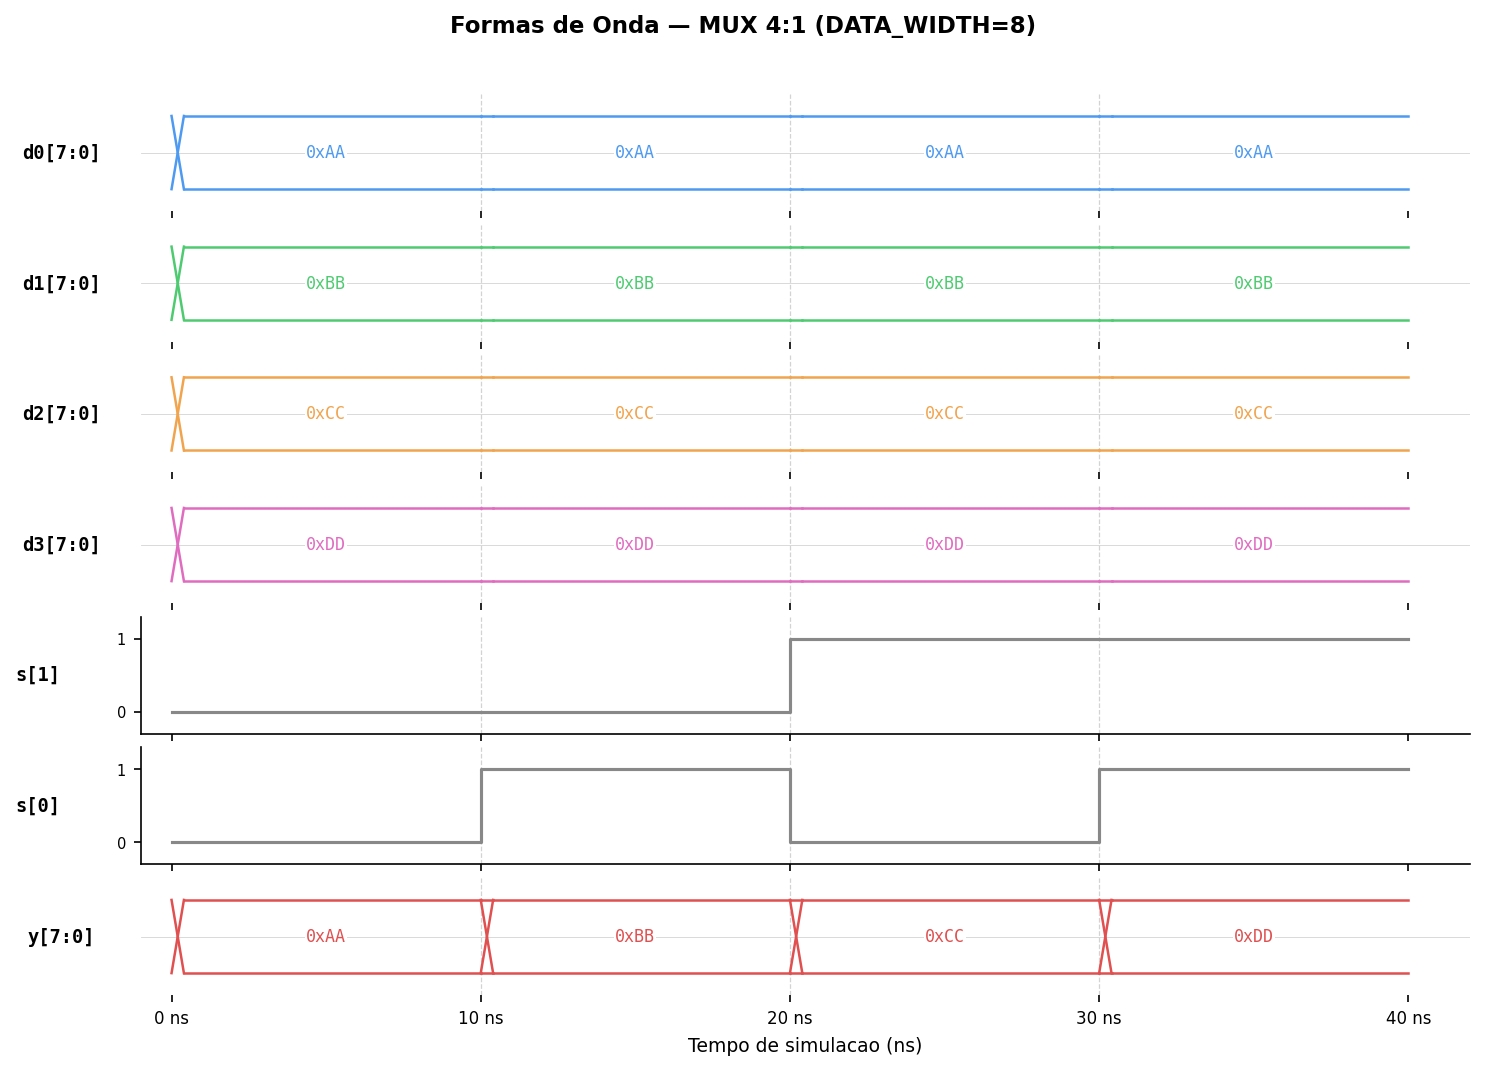
\includegraphics[width=0.95\linewidth]{fig_waveform_mux.png}
\caption{Formas de onda da simulacao do MUX 4-para-1. As entradas $D_0$--$D_3$
permanecem constantes em \texttt{0xAA}, \texttt{0xBB}, \texttt{0xCC} e \texttt{0xDD}
respectivamente. A cada $10\,\text{ns}$, o sinal de selecao $S[1:0]$ incrementa
de $00$ para $01$, $10$ e $11$, e a saida $Y$ adota exatamente o valor da entrada
correspondente. A transicao e instantanea (logica combinacional pura, sem clock).}
\label{fig:waveform}
\end{figure}

\subsection{Analise dos Resultados}

\begin{table}[H]
\centering
\small
\caption{Resumo dos vetores de teste aplicados e resultados obtidos.}
\label{tab:resultados}
\begin{tabular}{ccccccc}
\toprule
\textbf{Teste} & $S[1:0]$ & $D_0$ & $D_1$ & $D_2$ & $D_3$ & $Y$ (obtido)\\
\midrule
1 & \texttt{2'b00} & \texttt{0xAA} & \texttt{0xBB} & \texttt{0xCC} & \texttt{0xDD} & \texttt{0xAA} $\checkmark$ \\
2 & \texttt{2'b01} & \texttt{0xAA} & \texttt{0xBB} & \texttt{0xCC} & \texttt{0xDD} & \texttt{0xBB} $\checkmark$ \\
3 & \texttt{2'b10} & \texttt{0xAA} & \texttt{0xBB} & \texttt{0xCC} & \texttt{0xDD} & \texttt{0xCC} $\checkmark$ \\
4 & \texttt{2'b11} & \texttt{0xAA} & \texttt{0xBB} & \texttt{0xCC} & \texttt{0xDD} & \texttt{0xDD} $\checkmark$ \\
\midrule
\multicolumn{6}{l}{\textbf{Cobertura total: 4/4 (100\%) -- Resultado: APROVADO}} & $\checkmark$ \\
\bottomrule
\end{tabular}
\end{table}

Os resultados confirmam a precisao funcional do modulo \texttt{mux\_4\_to\_1}:

\begin{itemize}
  \item \textbf{Roteamento correto:} Para cada valor de $S$, a saida $Y$ assumiu
        exatamente o valor da entrada correspondente ($D_0$--$D_3$), em acordo com
        a tabela-verdade do MUX 4:1 (Tabela~\ref{tab:verdade}).
  \item \textbf{Comportamento combinacional:} A propagacao da saida ocorre sem atraso
        de clock, confirmando a semantica do bloco \texttt{always\_comb}.
  \item \textbf{Parametrizacao verificada:} Com \texttt{DATA\_WIDTH = 8}, todas as
        8 linhas de dados foram corretamente roteadas, validando o uso do parametro.
  \item \textbf{Temporizacao:} A execucao total foi de $40\,\text{ns}$ (4 testes
        $\times$ $10\,\text{ns}$), correspondendo a $40\,000$ unidades de tempo da
        \textit{timescale} \texttt{1ns/1ps}.
\end{itemize}

%% ─── 6. CONCLUSOES ─────────────────────────────────────────────────────────
\section{Conclusoes}

A verificacao funcional atestou a precisao da logica combinacional implementada
no modulo MUX 4:1. Os dados extraidos do console de simulacao e do visualizador
de formas de onda evidenciaram a correlacao exata entre as transicoes do sinal de
selecao e o respectivo roteamento das entradas de dados para a saida.

O projeto demonstrou na pratica os seguintes conceitos de SystemVerilog:

\begin{enumerate}
  \item \textbf{Parametrizacao com \texttt{\#(parameter int DATA\_WIDTH)}:}
        Permite a reutilizacao do modulo para qualquer largura de barramento
        sem alteracao do codigo -- um requisito de nivel industrial.
  \item \textbf{Bloco \texttt{always\_comb}:} Garante sintese como logica
        combinacional pura, sem risco de latch involuntario.
  \item \textbf{Construtor \texttt{unique case}:} Adiciona verificacao de cobertura
        completa pelo sintetizador, tornando o codigo mais robusto.
  \item \textbf{Testbench com verificacao automatica:} A tarefa \texttt{testa\_mux}
        com contagem de erros e relatorio PASS/FAIL e a abordagem correta para
        validacao de \textit{designs} RTL em ambiente profissional.
\end{enumerate}

A utilizacao do \textit{testbench} para a aplicacao de vetores de teste nas 4
combinacoes de selecao validou a integridade do codigo RTL frente aos requisitos
operacionais definidos na especificacao, confirmando a correta operacao do circuito
e a conclusao bem-sucedida da atividade proposta.

%% ─── REFERENCIAS ────────────────────────────────────────────────────────────
\renewcommand{\refname}{Referencias Bibliograficas}
\begin{thebibliography}{99}

\bibitem{ieee1800}
IEEE STANDARDS ASSOCIATION.
\textit{IEEE Standard for SystemVerilog -- Unified Hardware Design, Specification,
and Verification Language}. IEEE Std 1800-2012. New York: IEEE, 2013.

\bibitem{edaplayground}
EDA PLAYGROUND.
\textit{EDA Playground -- Online HDL Simulator}.
Disponivel em: \url{https://www.edaplayground.com/}.
Acesso em: 1 mai.\ 2026.

\bibitem{iverilog}
WILLIAMS, S.
\textit{Icarus Verilog -- Open-Source Verilog Simulator}. v12.0, 2023.
Disponivel em: \url{http://iverilog.icarus.com/}.
Acesso em: 12 mai.\ 2026.

\bibitem{razavi2015}
RAZAVI, Behzad.
\textit{Design of Analog CMOS Integrated Circuits}. 2.~ed.
McGraw-Hill Education, New York, 2016.

\bibitem{brown2014}
BROWN, S.; VRANESIC, Z.
\textit{Fundamentals of Digital Logic with Verilog Design}. 3.~ed.
McGraw-Hill Education, New York, 2014.

\end{thebibliography}

\end{document}
